\documentclass[11pt]{standalone}
\usepackage{amssymb}
\usepackage{amsmath}
\usepackage[no-math]{fontspec}
\usepackage{unicode-math}
\usepackage{libertinus}
\usepackage{pgf,xcolor}
\usepackage{tikz}
\usetikzlibrary{arrows.meta, backgrounds}
\usepackage{pgfplots}
\pgfplotsset{compat=newest}

\definecolor{my_darkgray}{HTML}{484949}
\definecolor{my_lightgray}{HTML}{F3F4F4}
\definecolor{my_darkblue}{HTML}{005A94}
\definecolor{my_lightblue}{HTML}{CCDEE9}
\definecolor{my_yellow}{HTML}{FFEC7F}
\definecolor{my_red}{HTML}{E60000}
\definecolor{my_orange}{HTML}{E87846}

\begin{document}

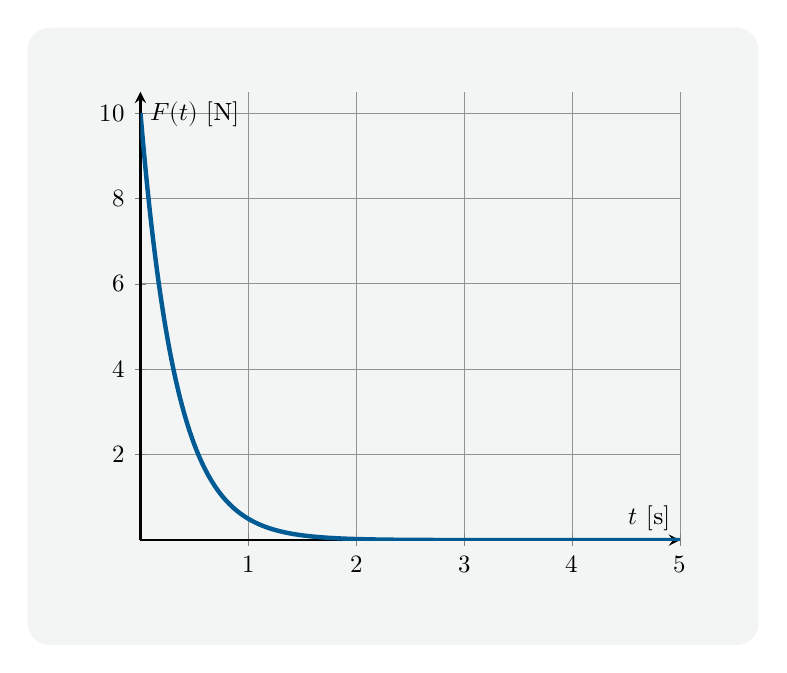
\begin{tikzpicture}[
    show background rectangle,
    background rectangle/.style={fill=my_lightgray, rounded corners=8pt},
    inner frame sep=0.8cm
]

\begin{axis}[
    axis lines = center,
    axis line style = {thick},
    xlabel = {$t~[\text{s}]$},
    ylabel = {$F(t)~[\text{N}]$},
    xlabel style = {font=\small},
    ylabel style = {font=\small},
    grid = both,
    minor grid style = {draw=my_lightblue},
    major grid style = {draw=my_darkgray!60},
    xmin = 0,
    xmax = 5,
    ymin = 0,
    ymax = 10.5,
    ticklabel style = {font=\small},
    % axis equal is omitted here, um den Abfall der Exponentialfunktion
    % in y-Richtung deutlicher sichtbar zu machen.
]

\addplot[
    draw = my_darkblue,
    ultra thick,
    samples = 300,
    domain = 0:5
]
{10*exp(-3*x)};

\end{axis}

\end{tikzpicture}

\end{document}